% ============================================================
% CHAPTER 5: Sprint 7 & Sprint 8 — Polish, Testing & Deployment
% ============================================================
% ADD THIS TO main.tex AFTER COMPLETING SPRINT 7 & 8
% Uncomment: % ============================================================
% CHAPTER 5: Sprint 7 & Sprint 8 — Polish, Testing & Deployment
% ============================================================
% ADD THIS TO main.tex AFTER COMPLETING SPRINT 7 & 8
% Uncomment: % ============================================================
% CHAPTER 5: Sprint 7 & Sprint 8 — Polish, Testing & Deployment
% ============================================================
% ADD THIS TO main.tex AFTER COMPLETING SPRINT 7 & 8
% Uncomment: % ============================================================
% CHAPTER 5: Sprint 7 & Sprint 8 — Polish, Testing & Deployment
% ============================================================
% ADD THIS TO main.tex AFTER COMPLETING SPRINT 7 & 8
% Uncomment: \input{chapters/chapter5}
% ============================================================
\chapter{Sprint 7 \& Sprint 8: Testing, Deployment and Finalization}

\section{Introduction}

This final chapter covers the last two sprints of the project. Sprint 7 focuses on notifications, UI polish, and comprehensive integration testing. Sprint 8 handles production deployment, final documentation, and presentation preparation.

% ============================================================
% SPRINT 7
% ============================================================
\section{Sprint 7: Notifications \& Integration Testing}

\sprintcard{7}{Notifications \& Integration Testing}{Implement notification system, polish the UI, and conduct thorough integration testing across all features.}

\subsection{Sprint Backlog}

\begin{longtable}{|c|p{5cm}|c|c|c|}
\hline
\rowcolor{blue!15}
\textbf{Task ID} & \textbf{Task} & \textbf{Assignee} & \textbf{Est.} & \textbf{Status} \\
\hline
\endhead
T-7.1 & Notification service (backend) & DSI & 4h & Done \\
\hline
T-7.2 & In-app notification UI & DSI & 3h & Done \\
\hline
T-7.3 & Error handling improvements & DSI & 4h & Done \\
\hline
T-7.4 & UI polish (loading, animations) & DSI & 5h & Done \\
\hline
T-7.5 & Integration testing & DSI & 6h & Done \\
\hline
T-7.6 & Bug fixes & DSI & 4h & Done \\
\hline
T-7.7 & Server end-to-end testing & RSI & 6h & Done \\
\hline
T-7.8 & Security stress testing & RSI & 4h & Done \\
\hline
T-7.9 & Infrastructure documentation & RSI & 4h & Done \\
\hline
\caption{Sprint 7 backlog}
\label{tab:sprint7-backlog}
\end{longtable}

\subsection{Sequence Diagram — Notification Flow}

\begin{figure}[H]
\centering
\begin{tikzpicture}[font=\small]
  \node (worker) at (0, 0) {\textbf{Worker}};
  \node (nats) at (3.5, 0) {\textbf{JetStream}};
  \node (notif) at (7, 0) {\textbf{Notif Service}};
  \node (db) at (10.5, 0) {\textbf{Database}};
  \node (front) at (14, 0) {\textbf{Frontend}};
  
  \draw[dashed] (worker) -- (0, -7);
  \draw[dashed] (nats) -- (3.5, -7);
  \draw[dashed] (notif) -- (7, -7);
  \draw[dashed] (db) -- (10.5, -7);
  \draw[dashed] (front) -- (14, -7);
  
  \draw[->, thick] (0, -1) -- node[above, font=\tiny] {VM status changed} (3.5, -1);
  \draw[->, thick] (3.5, -2) -- node[above, font=\tiny] {Consume event} (7, -2);
  \draw[->, thick] (7, -3) -- node[above, font=\tiny] {Save notification} (10.5, -3);
  \draw[<-, thick] (7, -3.5) -- node[above, font=\tiny] {Saved} (10.5, -3.5);
  \draw[->, thick] (7, -4.5) -- node[above, font=\tiny] {Push notification} (14, -4.5);
  \draw[->, thick] (14, -5.5) -- node[right, font=\tiny] {Show toast};
\end{tikzpicture}
\caption{Sequence diagram — Notification flow}
\label{fig:seq-notification}
\end{figure}

\subsection{Integration Testing Results}

The following table summarizes the integration testing results for all major features:

\begin{longtable}{|c|p{5cm}|c|p{3cm}|}
\hline
\rowcolor{blue!15}
\textbf{\#} & \textbf{Test Scenario} & \textbf{Result} & \textbf{Notes} \\
\hline
\endhead
1 & User registration & \textcolor{green!70!black}{PASS} & Email validation works \\
\hline
2 & User login with JWT & \textcolor{green!70!black}{PASS} & Tokens generated correctly \\
\hline
3 & Token refresh & \textcolor{green!70!black}{PASS} & Seamless refresh \\
\hline
4 & Create VM within quota & \textcolor{green!70!black}{PASS} & VM provisioned in OpenNebula \\
\hline
5 & Create VM over quota & \textcolor{green!70!black}{PASS} & 403 returned correctly \\
\hline
6 & Stop running VM & \textcolor{green!70!black}{PASS} & Status updates via JetStream \\
\hline
7 & Start stopped VM & \textcolor{green!70!black}{PASS} & VM resumes correctly \\
\hline
8 & Reboot VM & \textcolor{green!70!black}{PASS} & Graceful reboot \\
\hline
9 & Delete VM & \textcolor{green!70!black}{PASS} & Quota updated \\
\hline
10 & Upgrade plan & \textcolor{green!70!black}{PASS} & Quota limits updated \\
\hline
11 & Admin delete user & \textcolor{green!70!black}{PASS} & User's VMs cleaned up \\
\hline
12 & Admin manage VMs & \textcolor{green!70!black}{PASS} & Force operations work \\
\hline
13 & VM status notification & \textcolor{green!70!black}{PASS} & Real-time notifications \\
\hline
14 & Web terminal (CLI) access & \textcolor{green!70!black}{PASS} & xterm.js connects via WebSocket SSH \\
\hline
15 & SSH key add/delete & \textcolor{green!70!black}{PASS} & Keys stored and used for VM auth \\
\hline
16 & Firewall blocks unauthorized & \textcolor{green!70!black}{PASS} & Only allowed ports open \\
\hline
\caption{Integration testing results}
\label{tab:test-results}
\end{longtable}

\subsection{Implementation Screenshots}

\begin{figure}[H]
\centering
\fbox{\parbox{0.9\textwidth}{\centering\vspace{3cm}\textit{Insert notification panel screenshot}\vspace{3cm}}}
\caption{In-app notification panel}
\label{fig:notifications}
\end{figure}

\subsection{Sprint 7 Review}

At the end of Sprint 7:
\begin{itemize}
  \item Notification service delivering real-time VM status updates.
  \item UI polish with loading skeletons, animations, and error messages.
  \item All 16 integration tests passing.
  \item Bug fixes applied for edge cases.
  \item Server security stress testing completed.
  \item Infrastructure documentation finalized.
\end{itemize}


% ============================================================
% SPRINT 8
% ============================================================
\section{Sprint 8: Deployment \& Finalization}

\sprintcard{8}{Deployment \& Finalization}{Deploy the complete platform on the Ubuntu Server, finalize documentation, and prepare the project presentation.}

\subsection{Sprint Backlog}

\begin{longtable}{|c|p{5cm}|c|c|c|}
\hline
\rowcolor{blue!15}
\textbf{Task ID} & \textbf{Task} & \textbf{Assignee} & \textbf{Est.} & \textbf{Status} \\
\hline
\endhead
T-8.1 & Production Docker builds & DSI & 4h & Done \\
\hline
T-8.2 & Deploy all services & DSI & 4h & Done \\
\hline
T-8.3 & Final testing on server & DSI & 4h & Done \\
\hline
T-8.4 & Report finalization & DSI & 6h & Done \\
\hline
T-8.5 & Presentation preparation & DSI & 4h & Done \\
\hline
T-8.6 & Production server config & RSI & 4h & Done \\
\hline
T-8.7 & Deployment verification & RSI & 4h & Done \\
\hline
T-8.8 & Report (infra sections) & RSI & 6h & Done \\
\hline
T-8.9 & Presentation preparation & RSI & 4h & Done \\
\hline
\caption{Sprint 8 backlog}
\label{tab:sprint8-backlog}
\end{longtable}

\subsection{Deployment Architecture}

\begin{figure}[H]
\centering
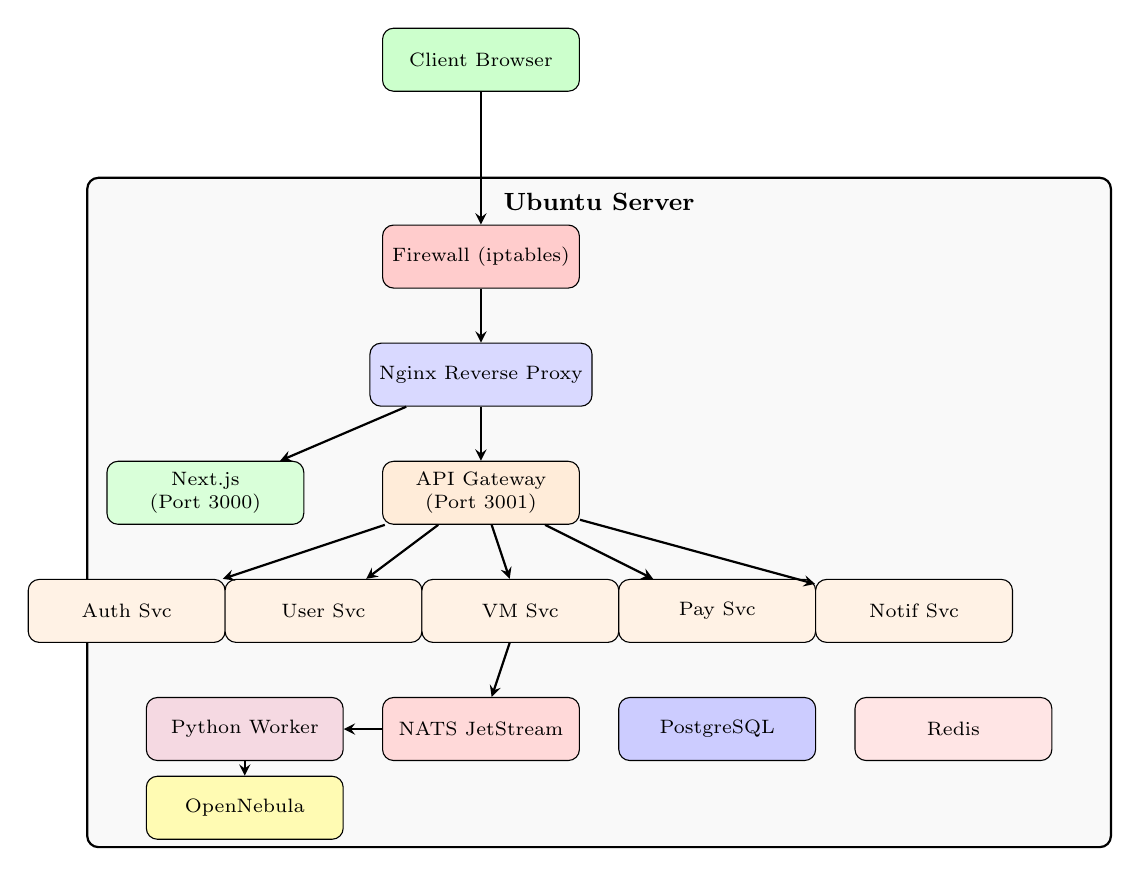
\begin{tikzpicture}[
  box/.style={draw, rounded corners, minimum width=2.5cm, minimum height=0.8cm, align=center, font=\scriptsize},
  container/.style={draw, dashed, rounded corners, inner sep=0.3cm},
  arrow/.style={->, thick, >=stealth}
]
  % Client
  \node[box, fill=green!20] (client) at (0, 4) {Client Browser};
  
  % Server boundary
  \draw[thick, rounded corners, fill=gray!5] (-5, -6) rectangle (8, 2.5);
  \node[font=\small\bfseries] at (1.5, 2.2) {Ubuntu Server};
  
  % Firewall
  \node[box, fill=red!20] (fw) at (0, 1.5) {Firewall (iptables)};
  
  % Docker containers
  \node[box, fill=blue!15] (nginx) at (0, 0) {Nginx Reverse Proxy};
  
  \node[box, fill=green!15] (next) at (-3.5, -1.5) {Next.js\\(Port 3000)};
  \node[box, fill=orange!15] (gate) at (0, -1.5) {API Gateway\\(Port 3001)};
  
  \node[box, fill=orange!10] (auth) at (-4.5, -3) {Auth Svc};
  \node[box, fill=orange!10] (usersvc) at (-2, -3) {User Svc};
  \node[box, fill=orange!10] (vmsvc) at (0.5, -3) {VM Svc};
  \node[box, fill=orange!10] (paysvc) at (3, -3) {Pay Svc};
  \node[box, fill=orange!10] (notifsvc) at (5.5, -3) {Notif Svc};
  
  \node[box, fill=purple!15] (worker) at (-3, -4.5) {Python Worker};
  \node[box, fill=red!15] (nats) at (0, -4.5) {NATS JetStream};
  \node[box, fill=blue!20] (pg) at (3, -4.5) {PostgreSQL};
  \node[box, fill=red!10] (redis) at (6, -4.5) {Redis};
  
  % OpenNebula
  \node[box, fill=yellow!30] (one) at (-3, -5.5) {OpenNebula};
  
  % Arrows
  \draw[arrow] (client) -- (fw);
  \draw[arrow] (fw) -- (nginx);
  \draw[arrow] (nginx) -- (next);
  \draw[arrow] (nginx) -- (gate);
  \draw[arrow] (gate) -- (auth);
  \draw[arrow] (gate) -- (usersvc);
  \draw[arrow] (gate) -- (vmsvc);
  \draw[arrow] (gate) -- (paysvc);
  \draw[arrow] (gate) -- (notifsvc);
  \draw[arrow] (vmsvc) -- (nats);
  \draw[arrow] (nats) -- (worker);
  \draw[arrow] (worker) -- (one);
\end{tikzpicture}
\caption{Deployment architecture}
\label{fig:deployment}
\end{figure}

\subsection{Network Topology}

\begin{figure}[H]
\centering
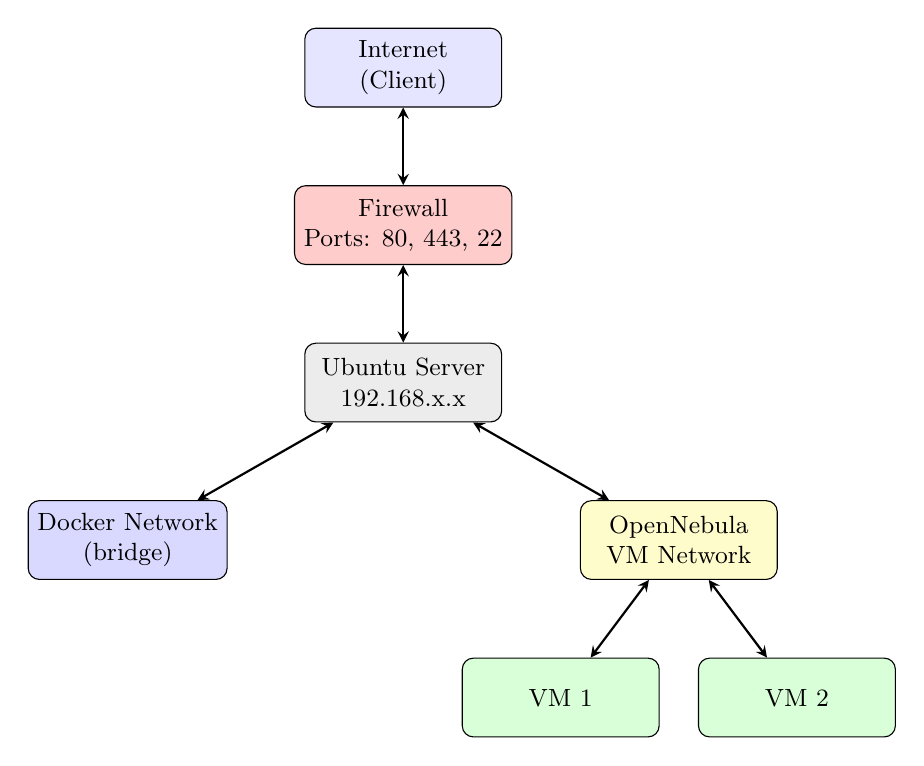
\begin{tikzpicture}[
  box/.style={draw, rounded corners, minimum width=2.5cm, minimum height=1cm, align=center, font=\small},
  arrow/.style={<->, thick, >=stealth}
]
  % Internet
  \node[box, fill=blue!10] (internet) at (0, 3) {Internet\\(Client)};
  
  % Firewall
  \node[box, fill=red!20] (fw) at (0, 1) {Firewall\\Ports: 80, 443, 22};
  
  % Server
  \node[box, fill=gray!15] (server) at (0, -1) {Ubuntu Server\\192.168.x.x};
  
  % Docker Network
  \node[box, fill=blue!15] (docker) at (-3.5, -3) {Docker Network\\(bridge)};
  
  % VM Network
  \node[box, fill=yellow!20] (vmnet) at (3.5, -3) {OpenNebula\\VM Network};
  
  % VMs
  \node[box, fill=green!15] (vm1) at (2, -5) {VM 1};
  \node[box, fill=green!15] (vm2) at (5, -5) {VM 2};
  
  \draw[arrow] (internet) -- (fw);
  \draw[arrow] (fw) -- (server);
  \draw[arrow] (server) -- (docker);
  \draw[arrow] (server) -- (vmnet);
  \draw[arrow] (vmnet) -- (vm1);
  \draw[arrow] (vmnet) -- (vm2);
\end{tikzpicture}
\caption{Network topology diagram}
\label{fig:network-topology}
\end{figure}

\subsection{Implementation Screenshots}

\begin{figure}[H]
\centering
\fbox{\parbox{0.9\textwidth}{\centering\vspace{3cm}\textit{Insert deployed platform screenshot (complete dashboard)}\vspace{3cm}}}
\caption{Deployed platform — User dashboard}
\label{fig:deployed-dashboard}
\end{figure}

\begin{figure}[H]
\centering
\fbox{\parbox{0.9\textwidth}{\centering\vspace{3cm}\textit{Insert Docker containers running screenshot}\vspace{3cm}}}
\caption{Docker containers running on the server}
\label{fig:docker-running}
\end{figure}

\subsection{Sprint 8 Review}

At the end of Sprint 8:
\begin{itemize}
  \item All services deployed via Docker Compose on Ubuntu Server.
  \item Production-optimized Docker builds (multi-stage).
  \item Nginx reverse proxy configured.
  \item Final smoke tests passed on deployed platform.
  \item Report completed and reviewed.
  \item Presentation slides and demo script prepared.
\end{itemize}

% ============================================================
\section{Conclusion}

In this final chapter, we completed the platform development with notification features, thorough testing, and full deployment. Sprint 7 ensured the platform's quality through integration testing and UI refinements. Sprint 8 delivered the production deployment with Docker, configured the server with proper security, and prepared all project deliverables.

The CloudVM platform is now fully functional, allowing users to create and manage virtual machines through a modern web interface, with secure authentication, quota management, and payment processing.

% ============================================================
% GENERAL CONCLUSION (to be added to main.tex)
% ============================================================
% Uncomment the following in main.tex at the end:

% \chapter*{General Conclusion}
% \addcontentsline{toc}{chapter}{General Conclusion}
% 
% Throughout this project, we designed and developed CloudVM — a comprehensive 
% cloud virtual machine management platform. The project was carried out within 
% the Readdly startup over a period of 8 weeks, following the Agile/Scrum methodology.
%
% The platform successfully delivers the following capabilities:
% \begin{itemize}
%   \item A modern, responsive web interface for VM management
%   \item Secure authentication with JWT and role-based access control
%   \item Full VM lifecycle management (create, start, stop, reboot, delete)
%   \item Web-based CLI terminal access to VMs (Phase~1) using xterm.js and WebSocket SSH proxy
%   \item SSH key management for secure VM authentication
%   \item Asynchronous processing through a Python worker and NATS JetStream
%   \item Quota enforcement and payment processing for plan upgrades
%   \item Server-side security with OpenNebula and firewall configuration
% \end{itemize}
%
% This project allowed us to apply the knowledge gained during our studies at 
% ISET Mahdia in a real-world context. We gained hands-on experience with 
% microservices architecture, containerization, cloud computing, and modern 
% web development practices.
%
% As future improvements, we envision:
% \begin{itemize}
%   \item \textbf{Phase~2 --- Full Desktop Streaming:} Upgrading VM access from the current CLI terminal to full graphical desktop streaming using VNC/noVNC, allowing users to interact with the VM's GUI (Windows desktop, Linux desktop environment) directly in the browser
%   \item Implementing auto-scaling and load balancing
%   \item Adding support for Kubernetes-based container orchestration
%   \item Deploying on public cloud infrastructure for wider accessibility
%   \item Adding more payment providers and subscription models
% \end{itemize}

% ============================================================
\chapter{Sprint 7 \& Sprint 8: Testing, Deployment and Finalization}

\section{Introduction}

This final chapter covers the last two sprints of the project. Sprint 7 focuses on notifications, UI polish, and comprehensive integration testing. Sprint 8 handles production deployment, final documentation, and presentation preparation.

% ============================================================
% SPRINT 7
% ============================================================
\section{Sprint 7: Notifications \& Integration Testing}

\sprintcard{7}{Notifications \& Integration Testing}{Implement notification system, polish the UI, and conduct thorough integration testing across all features.}

\subsection{Sprint Backlog}

\begin{longtable}{|c|p{5cm}|c|c|c|}
\hline
\rowcolor{blue!15}
\textbf{Task ID} & \textbf{Task} & \textbf{Assignee} & \textbf{Est.} & \textbf{Status} \\
\hline
\endhead
T-7.1 & Notification service (backend) & DSI & 4h & Done \\
\hline
T-7.2 & In-app notification UI & DSI & 3h & Done \\
\hline
T-7.3 & Error handling improvements & DSI & 4h & Done \\
\hline
T-7.4 & UI polish (loading, animations) & DSI & 5h & Done \\
\hline
T-7.5 & Integration testing & DSI & 6h & Done \\
\hline
T-7.6 & Bug fixes & DSI & 4h & Done \\
\hline
T-7.7 & Server end-to-end testing & RSI & 6h & Done \\
\hline
T-7.8 & Security stress testing & RSI & 4h & Done \\
\hline
T-7.9 & Infrastructure documentation & RSI & 4h & Done \\
\hline
\caption{Sprint 7 backlog}
\label{tab:sprint7-backlog}
\end{longtable}

\subsection{Sequence Diagram — Notification Flow}

\begin{figure}[H]
\centering
\begin{tikzpicture}[font=\small]
  \node (worker) at (0, 0) {\textbf{Worker}};
  \node (nats) at (3.5, 0) {\textbf{JetStream}};
  \node (notif) at (7, 0) {\textbf{Notif Service}};
  \node (db) at (10.5, 0) {\textbf{Database}};
  \node (front) at (14, 0) {\textbf{Frontend}};
  
  \draw[dashed] (worker) -- (0, -7);
  \draw[dashed] (nats) -- (3.5, -7);
  \draw[dashed] (notif) -- (7, -7);
  \draw[dashed] (db) -- (10.5, -7);
  \draw[dashed] (front) -- (14, -7);
  
  \draw[->, thick] (0, -1) -- node[above, font=\tiny] {VM status changed} (3.5, -1);
  \draw[->, thick] (3.5, -2) -- node[above, font=\tiny] {Consume event} (7, -2);
  \draw[->, thick] (7, -3) -- node[above, font=\tiny] {Save notification} (10.5, -3);
  \draw[<-, thick] (7, -3.5) -- node[above, font=\tiny] {Saved} (10.5, -3.5);
  \draw[->, thick] (7, -4.5) -- node[above, font=\tiny] {Push notification} (14, -4.5);
  \draw[->, thick] (14, -5.5) -- node[right, font=\tiny] {Show toast};
\end{tikzpicture}
\caption{Sequence diagram — Notification flow}
\label{fig:seq-notification}
\end{figure}

\subsection{Integration Testing Results}

The following table summarizes the integration testing results for all major features:

\begin{longtable}{|c|p{5cm}|c|p{3cm}|}
\hline
\rowcolor{blue!15}
\textbf{\#} & \textbf{Test Scenario} & \textbf{Result} & \textbf{Notes} \\
\hline
\endhead
1 & User registration & \textcolor{green!70!black}{PASS} & Email validation works \\
\hline
2 & User login with JWT & \textcolor{green!70!black}{PASS} & Tokens generated correctly \\
\hline
3 & Token refresh & \textcolor{green!70!black}{PASS} & Seamless refresh \\
\hline
4 & Create VM within quota & \textcolor{green!70!black}{PASS} & VM provisioned in OpenNebula \\
\hline
5 & Create VM over quota & \textcolor{green!70!black}{PASS} & 403 returned correctly \\
\hline
6 & Stop running VM & \textcolor{green!70!black}{PASS} & Status updates via JetStream \\
\hline
7 & Start stopped VM & \textcolor{green!70!black}{PASS} & VM resumes correctly \\
\hline
8 & Reboot VM & \textcolor{green!70!black}{PASS} & Graceful reboot \\
\hline
9 & Delete VM & \textcolor{green!70!black}{PASS} & Quota updated \\
\hline
10 & Upgrade plan & \textcolor{green!70!black}{PASS} & Quota limits updated \\
\hline
11 & Admin delete user & \textcolor{green!70!black}{PASS} & User's VMs cleaned up \\
\hline
12 & Admin manage VMs & \textcolor{green!70!black}{PASS} & Force operations work \\
\hline
13 & VM status notification & \textcolor{green!70!black}{PASS} & Real-time notifications \\
\hline
14 & Web terminal (CLI) access & \textcolor{green!70!black}{PASS} & xterm.js connects via WebSocket SSH \\
\hline
15 & SSH key add/delete & \textcolor{green!70!black}{PASS} & Keys stored and used for VM auth \\
\hline
16 & Firewall blocks unauthorized & \textcolor{green!70!black}{PASS} & Only allowed ports open \\
\hline
\caption{Integration testing results}
\label{tab:test-results}
\end{longtable}

\subsection{Implementation Screenshots}

\begin{figure}[H]
\centering
\fbox{\parbox{0.9\textwidth}{\centering\vspace{3cm}\textit{Insert notification panel screenshot}\vspace{3cm}}}
\caption{In-app notification panel}
\label{fig:notifications}
\end{figure}

\subsection{Sprint 7 Review}

At the end of Sprint 7:
\begin{itemize}
  \item Notification service delivering real-time VM status updates.
  \item UI polish with loading skeletons, animations, and error messages.
  \item All 16 integration tests passing.
  \item Bug fixes applied for edge cases.
  \item Server security stress testing completed.
  \item Infrastructure documentation finalized.
\end{itemize}


% ============================================================
% SPRINT 8
% ============================================================
\section{Sprint 8: Deployment \& Finalization}

\sprintcard{8}{Deployment \& Finalization}{Deploy the complete platform on the Ubuntu Server, finalize documentation, and prepare the project presentation.}

\subsection{Sprint Backlog}

\begin{longtable}{|c|p{5cm}|c|c|c|}
\hline
\rowcolor{blue!15}
\textbf{Task ID} & \textbf{Task} & \textbf{Assignee} & \textbf{Est.} & \textbf{Status} \\
\hline
\endhead
T-8.1 & Production Docker builds & DSI & 4h & Done \\
\hline
T-8.2 & Deploy all services & DSI & 4h & Done \\
\hline
T-8.3 & Final testing on server & DSI & 4h & Done \\
\hline
T-8.4 & Report finalization & DSI & 6h & Done \\
\hline
T-8.5 & Presentation preparation & DSI & 4h & Done \\
\hline
T-8.6 & Production server config & RSI & 4h & Done \\
\hline
T-8.7 & Deployment verification & RSI & 4h & Done \\
\hline
T-8.8 & Report (infra sections) & RSI & 6h & Done \\
\hline
T-8.9 & Presentation preparation & RSI & 4h & Done \\
\hline
\caption{Sprint 8 backlog}
\label{tab:sprint8-backlog}
\end{longtable}

\subsection{Deployment Architecture}

\begin{figure}[H]
\centering
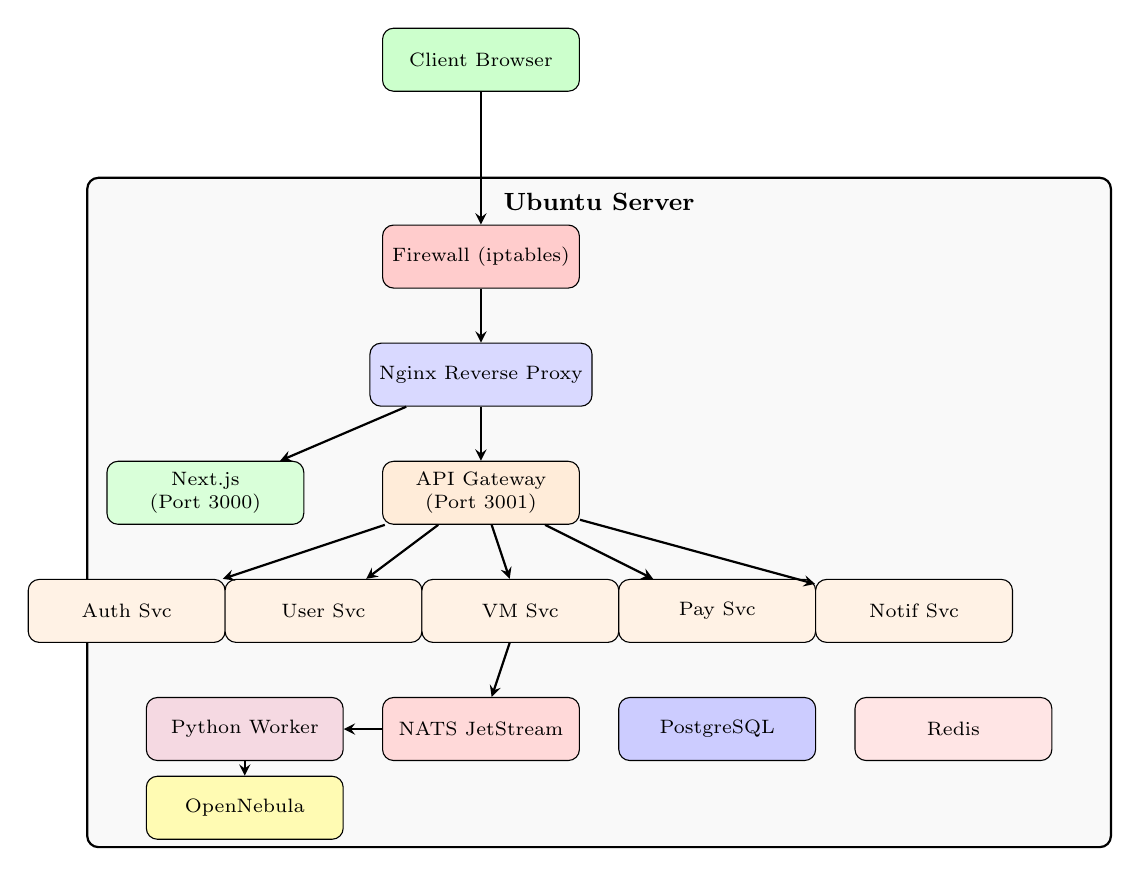
\begin{tikzpicture}[
  box/.style={draw, rounded corners, minimum width=2.5cm, minimum height=0.8cm, align=center, font=\scriptsize},
  container/.style={draw, dashed, rounded corners, inner sep=0.3cm},
  arrow/.style={->, thick, >=stealth}
]
  % Client
  \node[box, fill=green!20] (client) at (0, 4) {Client Browser};
  
  % Server boundary
  \draw[thick, rounded corners, fill=gray!5] (-5, -6) rectangle (8, 2.5);
  \node[font=\small\bfseries] at (1.5, 2.2) {Ubuntu Server};
  
  % Firewall
  \node[box, fill=red!20] (fw) at (0, 1.5) {Firewall (iptables)};
  
  % Docker containers
  \node[box, fill=blue!15] (nginx) at (0, 0) {Nginx Reverse Proxy};
  
  \node[box, fill=green!15] (next) at (-3.5, -1.5) {Next.js\\(Port 3000)};
  \node[box, fill=orange!15] (gate) at (0, -1.5) {API Gateway\\(Port 3001)};
  
  \node[box, fill=orange!10] (auth) at (-4.5, -3) {Auth Svc};
  \node[box, fill=orange!10] (usersvc) at (-2, -3) {User Svc};
  \node[box, fill=orange!10] (vmsvc) at (0.5, -3) {VM Svc};
  \node[box, fill=orange!10] (paysvc) at (3, -3) {Pay Svc};
  \node[box, fill=orange!10] (notifsvc) at (5.5, -3) {Notif Svc};
  
  \node[box, fill=purple!15] (worker) at (-3, -4.5) {Python Worker};
  \node[box, fill=red!15] (nats) at (0, -4.5) {NATS JetStream};
  \node[box, fill=blue!20] (pg) at (3, -4.5) {PostgreSQL};
  \node[box, fill=red!10] (redis) at (6, -4.5) {Redis};
  
  % OpenNebula
  \node[box, fill=yellow!30] (one) at (-3, -5.5) {OpenNebula};
  
  % Arrows
  \draw[arrow] (client) -- (fw);
  \draw[arrow] (fw) -- (nginx);
  \draw[arrow] (nginx) -- (next);
  \draw[arrow] (nginx) -- (gate);
  \draw[arrow] (gate) -- (auth);
  \draw[arrow] (gate) -- (usersvc);
  \draw[arrow] (gate) -- (vmsvc);
  \draw[arrow] (gate) -- (paysvc);
  \draw[arrow] (gate) -- (notifsvc);
  \draw[arrow] (vmsvc) -- (nats);
  \draw[arrow] (nats) -- (worker);
  \draw[arrow] (worker) -- (one);
\end{tikzpicture}
\caption{Deployment architecture}
\label{fig:deployment}
\end{figure}

\subsection{Network Topology}

\begin{figure}[H]
\centering
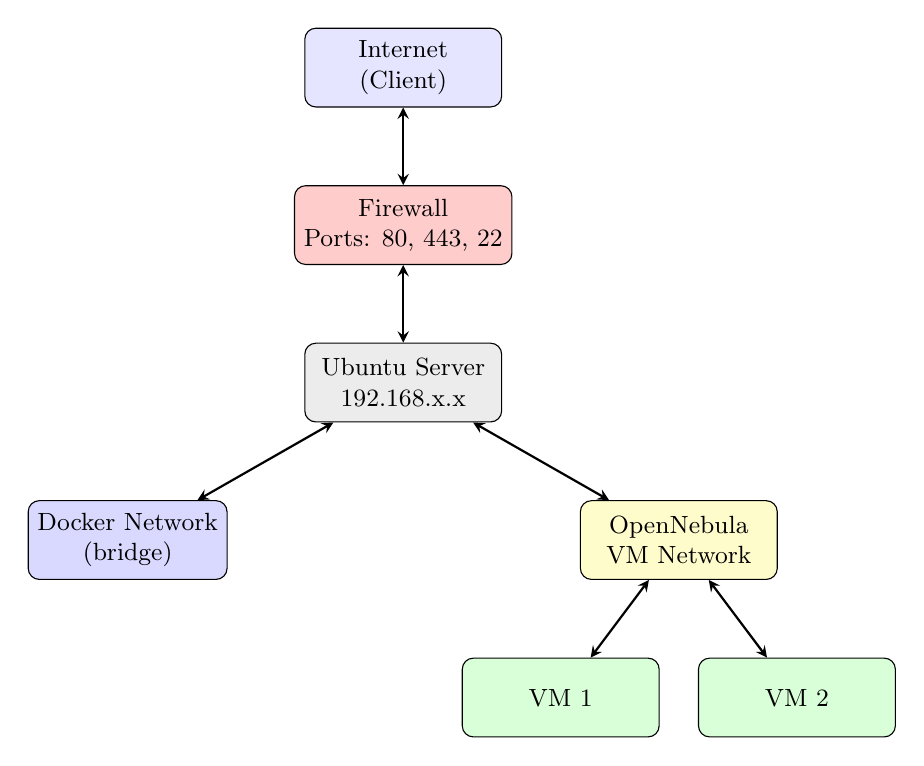
\begin{tikzpicture}[
  box/.style={draw, rounded corners, minimum width=2.5cm, minimum height=1cm, align=center, font=\small},
  arrow/.style={<->, thick, >=stealth}
]
  % Internet
  \node[box, fill=blue!10] (internet) at (0, 3) {Internet\\(Client)};
  
  % Firewall
  \node[box, fill=red!20] (fw) at (0, 1) {Firewall\\Ports: 80, 443, 22};
  
  % Server
  \node[box, fill=gray!15] (server) at (0, -1) {Ubuntu Server\\192.168.x.x};
  
  % Docker Network
  \node[box, fill=blue!15] (docker) at (-3.5, -3) {Docker Network\\(bridge)};
  
  % VM Network
  \node[box, fill=yellow!20] (vmnet) at (3.5, -3) {OpenNebula\\VM Network};
  
  % VMs
  \node[box, fill=green!15] (vm1) at (2, -5) {VM 1};
  \node[box, fill=green!15] (vm2) at (5, -5) {VM 2};
  
  \draw[arrow] (internet) -- (fw);
  \draw[arrow] (fw) -- (server);
  \draw[arrow] (server) -- (docker);
  \draw[arrow] (server) -- (vmnet);
  \draw[arrow] (vmnet) -- (vm1);
  \draw[arrow] (vmnet) -- (vm2);
\end{tikzpicture}
\caption{Network topology diagram}
\label{fig:network-topology}
\end{figure}

\subsection{Implementation Screenshots}

\begin{figure}[H]
\centering
\fbox{\parbox{0.9\textwidth}{\centering\vspace{3cm}\textit{Insert deployed platform screenshot (complete dashboard)}\vspace{3cm}}}
\caption{Deployed platform — User dashboard}
\label{fig:deployed-dashboard}
\end{figure}

\begin{figure}[H]
\centering
\fbox{\parbox{0.9\textwidth}{\centering\vspace{3cm}\textit{Insert Docker containers running screenshot}\vspace{3cm}}}
\caption{Docker containers running on the server}
\label{fig:docker-running}
\end{figure}

\subsection{Sprint 8 Review}

At the end of Sprint 8:
\begin{itemize}
  \item All services deployed via Docker Compose on Ubuntu Server.
  \item Production-optimized Docker builds (multi-stage).
  \item Nginx reverse proxy configured.
  \item Final smoke tests passed on deployed platform.
  \item Report completed and reviewed.
  \item Presentation slides and demo script prepared.
\end{itemize}

% ============================================================
\section{Conclusion}

In this final chapter, we completed the platform development with notification features, thorough testing, and full deployment. Sprint 7 ensured the platform's quality through integration testing and UI refinements. Sprint 8 delivered the production deployment with Docker, configured the server with proper security, and prepared all project deliverables.

The CloudVM platform is now fully functional, allowing users to create and manage virtual machines through a modern web interface, with secure authentication, quota management, and payment processing.

% ============================================================
% GENERAL CONCLUSION (to be added to main.tex)
% ============================================================
% Uncomment the following in main.tex at the end:

% \chapter*{General Conclusion}
% \addcontentsline{toc}{chapter}{General Conclusion}
% 
% Throughout this project, we designed and developed CloudVM — a comprehensive 
% cloud virtual machine management platform. The project was carried out within 
% the Readdly startup over a period of 8 weeks, following the Agile/Scrum methodology.
%
% The platform successfully delivers the following capabilities:
% \begin{itemize}
%   \item A modern, responsive web interface for VM management
%   \item Secure authentication with JWT and role-based access control
%   \item Full VM lifecycle management (create, start, stop, reboot, delete)
%   \item Web-based CLI terminal access to VMs (Phase~1) using xterm.js and WebSocket SSH proxy
%   \item SSH key management for secure VM authentication
%   \item Asynchronous processing through a Python worker and NATS JetStream
%   \item Quota enforcement and payment processing for plan upgrades
%   \item Server-side security with OpenNebula and firewall configuration
% \end{itemize}
%
% This project allowed us to apply the knowledge gained during our studies at 
% ISET Mahdia in a real-world context. We gained hands-on experience with 
% microservices architecture, containerization, cloud computing, and modern 
% web development practices.
%
% As future improvements, we envision:
% \begin{itemize}
%   \item \textbf{Phase~2 --- Full Desktop Streaming:} Upgrading VM access from the current CLI terminal to full graphical desktop streaming using VNC/noVNC, allowing users to interact with the VM's GUI (Windows desktop, Linux desktop environment) directly in the browser
%   \item Implementing auto-scaling and load balancing
%   \item Adding support for Kubernetes-based container orchestration
%   \item Deploying on public cloud infrastructure for wider accessibility
%   \item Adding more payment providers and subscription models
% \end{itemize}

% ============================================================
\chapter{Sprint 7 \& Sprint 8: Testing, Deployment and Finalization}

\section{Introduction}

This final chapter covers the last two sprints of the project. Sprint 7 focuses on notifications, UI polish, and comprehensive integration testing. Sprint 8 handles production deployment, final documentation, and presentation preparation.

% ============================================================
% SPRINT 7
% ============================================================
\section{Sprint 7: Notifications \& Integration Testing}

\sprintcard{7}{Notifications \& Integration Testing}{Implement notification system, polish the UI, and conduct thorough integration testing across all features.}

\subsection{Sprint Backlog}

\begin{longtable}{|c|p{5cm}|c|c|c|}
\hline
\rowcolor{blue!15}
\textbf{Task ID} & \textbf{Task} & \textbf{Assignee} & \textbf{Est.} & \textbf{Status} \\
\hline
\endhead
T-7.1 & Notification service (backend) & DSI & 4h & Done \\
\hline
T-7.2 & In-app notification UI & DSI & 3h & Done \\
\hline
T-7.3 & Error handling improvements & DSI & 4h & Done \\
\hline
T-7.4 & UI polish (loading, animations) & DSI & 5h & Done \\
\hline
T-7.5 & Integration testing & DSI & 6h & Done \\
\hline
T-7.6 & Bug fixes & DSI & 4h & Done \\
\hline
T-7.7 & Server end-to-end testing & RSI & 6h & Done \\
\hline
T-7.8 & Security stress testing & RSI & 4h & Done \\
\hline
T-7.9 & Infrastructure documentation & RSI & 4h & Done \\
\hline
\caption{Sprint 7 backlog}
\label{tab:sprint7-backlog}
\end{longtable}

\subsection{Sequence Diagram — Notification Flow}

\begin{figure}[H]
\centering
\begin{tikzpicture}[font=\small]
  \node (worker) at (0, 0) {\textbf{Worker}};
  \node (nats) at (3.5, 0) {\textbf{JetStream}};
  \node (notif) at (7, 0) {\textbf{Notif Service}};
  \node (db) at (10.5, 0) {\textbf{Database}};
  \node (front) at (14, 0) {\textbf{Frontend}};
  
  \draw[dashed] (worker) -- (0, -7);
  \draw[dashed] (nats) -- (3.5, -7);
  \draw[dashed] (notif) -- (7, -7);
  \draw[dashed] (db) -- (10.5, -7);
  \draw[dashed] (front) -- (14, -7);
  
  \draw[->, thick] (0, -1) -- node[above, font=\tiny] {VM status changed} (3.5, -1);
  \draw[->, thick] (3.5, -2) -- node[above, font=\tiny] {Consume event} (7, -2);
  \draw[->, thick] (7, -3) -- node[above, font=\tiny] {Save notification} (10.5, -3);
  \draw[<-, thick] (7, -3.5) -- node[above, font=\tiny] {Saved} (10.5, -3.5);
  \draw[->, thick] (7, -4.5) -- node[above, font=\tiny] {Push notification} (14, -4.5);
  \draw[->, thick] (14, -5.5) -- node[right, font=\tiny] {Show toast};
\end{tikzpicture}
\caption{Sequence diagram — Notification flow}
\label{fig:seq-notification}
\end{figure}

\subsection{Integration Testing Results}

The following table summarizes the integration testing results for all major features:

\begin{longtable}{|c|p{5cm}|c|p{3cm}|}
\hline
\rowcolor{blue!15}
\textbf{\#} & \textbf{Test Scenario} & \textbf{Result} & \textbf{Notes} \\
\hline
\endhead
1 & User registration & \textcolor{green!70!black}{PASS} & Email validation works \\
\hline
2 & User login with JWT & \textcolor{green!70!black}{PASS} & Tokens generated correctly \\
\hline
3 & Token refresh & \textcolor{green!70!black}{PASS} & Seamless refresh \\
\hline
4 & Create VM within quota & \textcolor{green!70!black}{PASS} & VM provisioned in OpenNebula \\
\hline
5 & Create VM over quota & \textcolor{green!70!black}{PASS} & 403 returned correctly \\
\hline
6 & Stop running VM & \textcolor{green!70!black}{PASS} & Status updates via JetStream \\
\hline
7 & Start stopped VM & \textcolor{green!70!black}{PASS} & VM resumes correctly \\
\hline
8 & Reboot VM & \textcolor{green!70!black}{PASS} & Graceful reboot \\
\hline
9 & Delete VM & \textcolor{green!70!black}{PASS} & Quota updated \\
\hline
10 & Upgrade plan & \textcolor{green!70!black}{PASS} & Quota limits updated \\
\hline
11 & Admin delete user & \textcolor{green!70!black}{PASS} & User's VMs cleaned up \\
\hline
12 & Admin manage VMs & \textcolor{green!70!black}{PASS} & Force operations work \\
\hline
13 & VM status notification & \textcolor{green!70!black}{PASS} & Real-time notifications \\
\hline
14 & Web terminal (CLI) access & \textcolor{green!70!black}{PASS} & xterm.js connects via WebSocket SSH \\
\hline
15 & SSH key add/delete & \textcolor{green!70!black}{PASS} & Keys stored and used for VM auth \\
\hline
16 & Firewall blocks unauthorized & \textcolor{green!70!black}{PASS} & Only allowed ports open \\
\hline
\caption{Integration testing results}
\label{tab:test-results}
\end{longtable}

\subsection{Implementation Screenshots}

\begin{figure}[H]
\centering
\fbox{\parbox{0.9\textwidth}{\centering\vspace{3cm}\textit{Insert notification panel screenshot}\vspace{3cm}}}
\caption{In-app notification panel}
\label{fig:notifications}
\end{figure}

\subsection{Sprint 7 Review}

At the end of Sprint 7:
\begin{itemize}
  \item Notification service delivering real-time VM status updates.
  \item UI polish with loading skeletons, animations, and error messages.
  \item All 16 integration tests passing.
  \item Bug fixes applied for edge cases.
  \item Server security stress testing completed.
  \item Infrastructure documentation finalized.
\end{itemize}


% ============================================================
% SPRINT 8
% ============================================================
\section{Sprint 8: Deployment \& Finalization}

\sprintcard{8}{Deployment \& Finalization}{Deploy the complete platform on the Ubuntu Server, finalize documentation, and prepare the project presentation.}

\subsection{Sprint Backlog}

\begin{longtable}{|c|p{5cm}|c|c|c|}
\hline
\rowcolor{blue!15}
\textbf{Task ID} & \textbf{Task} & \textbf{Assignee} & \textbf{Est.} & \textbf{Status} \\
\hline
\endhead
T-8.1 & Production Docker builds & DSI & 4h & Done \\
\hline
T-8.2 & Deploy all services & DSI & 4h & Done \\
\hline
T-8.3 & Final testing on server & DSI & 4h & Done \\
\hline
T-8.4 & Report finalization & DSI & 6h & Done \\
\hline
T-8.5 & Presentation preparation & DSI & 4h & Done \\
\hline
T-8.6 & Production server config & RSI & 4h & Done \\
\hline
T-8.7 & Deployment verification & RSI & 4h & Done \\
\hline
T-8.8 & Report (infra sections) & RSI & 6h & Done \\
\hline
T-8.9 & Presentation preparation & RSI & 4h & Done \\
\hline
\caption{Sprint 8 backlog}
\label{tab:sprint8-backlog}
\end{longtable}

\subsection{Deployment Architecture}

\begin{figure}[H]
\centering
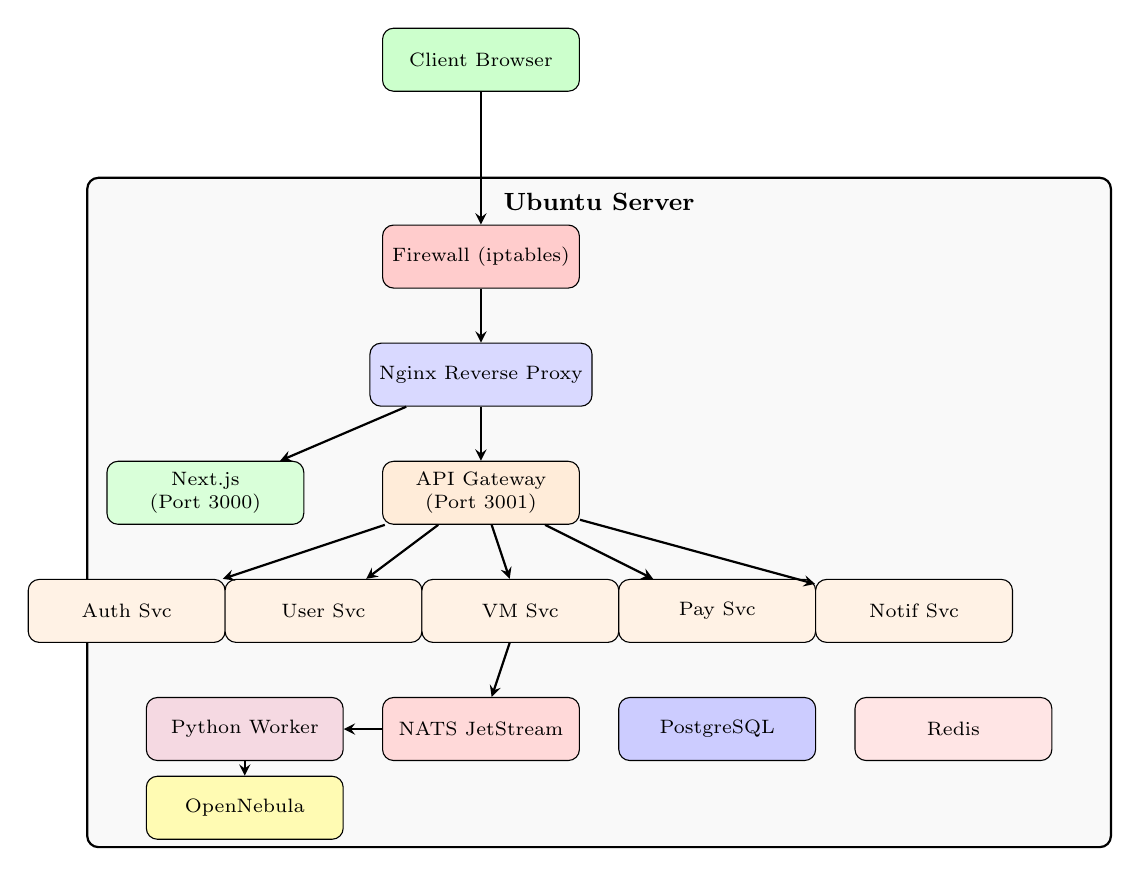
\begin{tikzpicture}[
  box/.style={draw, rounded corners, minimum width=2.5cm, minimum height=0.8cm, align=center, font=\scriptsize},
  container/.style={draw, dashed, rounded corners, inner sep=0.3cm},
  arrow/.style={->, thick, >=stealth}
]
  % Client
  \node[box, fill=green!20] (client) at (0, 4) {Client Browser};
  
  % Server boundary
  \draw[thick, rounded corners, fill=gray!5] (-5, -6) rectangle (8, 2.5);
  \node[font=\small\bfseries] at (1.5, 2.2) {Ubuntu Server};
  
  % Firewall
  \node[box, fill=red!20] (fw) at (0, 1.5) {Firewall (iptables)};
  
  % Docker containers
  \node[box, fill=blue!15] (nginx) at (0, 0) {Nginx Reverse Proxy};
  
  \node[box, fill=green!15] (next) at (-3.5, -1.5) {Next.js\\(Port 3000)};
  \node[box, fill=orange!15] (gate) at (0, -1.5) {API Gateway\\(Port 3001)};
  
  \node[box, fill=orange!10] (auth) at (-4.5, -3) {Auth Svc};
  \node[box, fill=orange!10] (usersvc) at (-2, -3) {User Svc};
  \node[box, fill=orange!10] (vmsvc) at (0.5, -3) {VM Svc};
  \node[box, fill=orange!10] (paysvc) at (3, -3) {Pay Svc};
  \node[box, fill=orange!10] (notifsvc) at (5.5, -3) {Notif Svc};
  
  \node[box, fill=purple!15] (worker) at (-3, -4.5) {Python Worker};
  \node[box, fill=red!15] (nats) at (0, -4.5) {NATS JetStream};
  \node[box, fill=blue!20] (pg) at (3, -4.5) {PostgreSQL};
  \node[box, fill=red!10] (redis) at (6, -4.5) {Redis};
  
  % OpenNebula
  \node[box, fill=yellow!30] (one) at (-3, -5.5) {OpenNebula};
  
  % Arrows
  \draw[arrow] (client) -- (fw);
  \draw[arrow] (fw) -- (nginx);
  \draw[arrow] (nginx) -- (next);
  \draw[arrow] (nginx) -- (gate);
  \draw[arrow] (gate) -- (auth);
  \draw[arrow] (gate) -- (usersvc);
  \draw[arrow] (gate) -- (vmsvc);
  \draw[arrow] (gate) -- (paysvc);
  \draw[arrow] (gate) -- (notifsvc);
  \draw[arrow] (vmsvc) -- (nats);
  \draw[arrow] (nats) -- (worker);
  \draw[arrow] (worker) -- (one);
\end{tikzpicture}
\caption{Deployment architecture}
\label{fig:deployment}
\end{figure}

\subsection{Network Topology}

\begin{figure}[H]
\centering
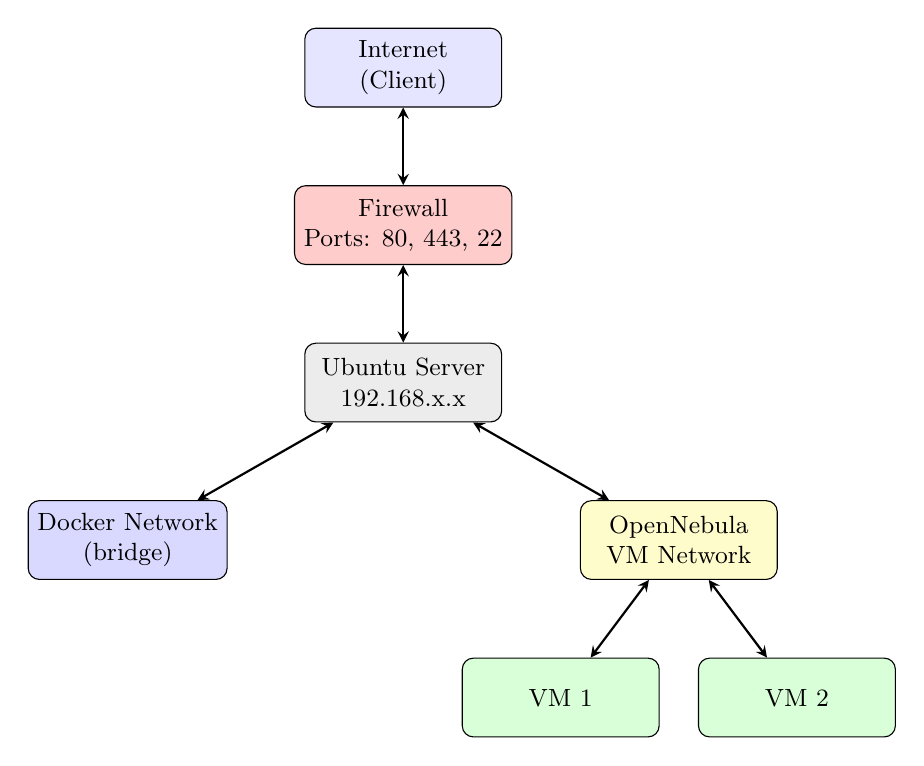
\begin{tikzpicture}[
  box/.style={draw, rounded corners, minimum width=2.5cm, minimum height=1cm, align=center, font=\small},
  arrow/.style={<->, thick, >=stealth}
]
  % Internet
  \node[box, fill=blue!10] (internet) at (0, 3) {Internet\\(Client)};
  
  % Firewall
  \node[box, fill=red!20] (fw) at (0, 1) {Firewall\\Ports: 80, 443, 22};
  
  % Server
  \node[box, fill=gray!15] (server) at (0, -1) {Ubuntu Server\\192.168.x.x};
  
  % Docker Network
  \node[box, fill=blue!15] (docker) at (-3.5, -3) {Docker Network\\(bridge)};
  
  % VM Network
  \node[box, fill=yellow!20] (vmnet) at (3.5, -3) {OpenNebula\\VM Network};
  
  % VMs
  \node[box, fill=green!15] (vm1) at (2, -5) {VM 1};
  \node[box, fill=green!15] (vm2) at (5, -5) {VM 2};
  
  \draw[arrow] (internet) -- (fw);
  \draw[arrow] (fw) -- (server);
  \draw[arrow] (server) -- (docker);
  \draw[arrow] (server) -- (vmnet);
  \draw[arrow] (vmnet) -- (vm1);
  \draw[arrow] (vmnet) -- (vm2);
\end{tikzpicture}
\caption{Network topology diagram}
\label{fig:network-topology}
\end{figure}

\subsection{Implementation Screenshots}

\begin{figure}[H]
\centering
\fbox{\parbox{0.9\textwidth}{\centering\vspace{3cm}\textit{Insert deployed platform screenshot (complete dashboard)}\vspace{3cm}}}
\caption{Deployed platform — User dashboard}
\label{fig:deployed-dashboard}
\end{figure}

\begin{figure}[H]
\centering
\fbox{\parbox{0.9\textwidth}{\centering\vspace{3cm}\textit{Insert Docker containers running screenshot}\vspace{3cm}}}
\caption{Docker containers running on the server}
\label{fig:docker-running}
\end{figure}

\subsection{Sprint 8 Review}

At the end of Sprint 8:
\begin{itemize}
  \item All services deployed via Docker Compose on Ubuntu Server.
  \item Production-optimized Docker builds (multi-stage).
  \item Nginx reverse proxy configured.
  \item Final smoke tests passed on deployed platform.
  \item Report completed and reviewed.
  \item Presentation slides and demo script prepared.
\end{itemize}

% ============================================================
\section{Conclusion}

In this final chapter, we completed the platform development with notification features, thorough testing, and full deployment. Sprint 7 ensured the platform's quality through integration testing and UI refinements. Sprint 8 delivered the production deployment with Docker, configured the server with proper security, and prepared all project deliverables.

The CloudVM platform is now fully functional, allowing users to create and manage virtual machines through a modern web interface, with secure authentication, quota management, and payment processing.

% ============================================================
% GENERAL CONCLUSION (to be added to main.tex)
% ============================================================
% Uncomment the following in main.tex at the end:

% \chapter*{General Conclusion}
% \addcontentsline{toc}{chapter}{General Conclusion}
% 
% Throughout this project, we designed and developed CloudVM — a comprehensive 
% cloud virtual machine management platform. The project was carried out within 
% the Readdly startup over a period of 8 weeks, following the Agile/Scrum methodology.
%
% The platform successfully delivers the following capabilities:
% \begin{itemize}
%   \item A modern, responsive web interface for VM management
%   \item Secure authentication with JWT and role-based access control
%   \item Full VM lifecycle management (create, start, stop, reboot, delete)
%   \item Web-based CLI terminal access to VMs (Phase~1) using xterm.js and WebSocket SSH proxy
%   \item SSH key management for secure VM authentication
%   \item Asynchronous processing through a Python worker and NATS JetStream
%   \item Quota enforcement and payment processing for plan upgrades
%   \item Server-side security with OpenNebula and firewall configuration
% \end{itemize}
%
% This project allowed us to apply the knowledge gained during our studies at 
% ISET Mahdia in a real-world context. We gained hands-on experience with 
% microservices architecture, containerization, cloud computing, and modern 
% web development practices.
%
% As future improvements, we envision:
% \begin{itemize}
%   \item \textbf{Phase~2 --- Full Desktop Streaming:} Upgrading VM access from the current CLI terminal to full graphical desktop streaming using VNC/noVNC, allowing users to interact with the VM's GUI (Windows desktop, Linux desktop environment) directly in the browser
%   \item Implementing auto-scaling and load balancing
%   \item Adding support for Kubernetes-based container orchestration
%   \item Deploying on public cloud infrastructure for wider accessibility
%   \item Adding more payment providers and subscription models
% \end{itemize}

% ============================================================
\chapter{Sprint 7 \& Sprint 8: Testing, Deployment and Finalization}

\section{Introduction}

This final chapter covers the last two sprints of the project. Sprint 7 focuses on notifications, UI polish, and comprehensive integration testing. Sprint 8 handles production deployment, final documentation, and presentation preparation.

% ============================================================
% SPRINT 7
% ============================================================
\section{Sprint 7: Notifications \& Integration Testing}

\sprintcard{7}{Notifications \& Integration Testing}{Implement notification system, polish the UI, and conduct thorough integration testing across all features.}

\subsection{Sprint Backlog}

\begin{longtable}{|c|p{5cm}|c|c|c|}
\hline
\rowcolor{blue!15}
\textbf{Task ID} & \textbf{Task} & \textbf{Assignee} & \textbf{Est.} & \textbf{Status} \\
\hline
\endhead
T-7.1 & Notification service (backend) & DSI & 4h & Done \\
\hline
T-7.2 & In-app notification UI & DSI & 3h & Done \\
\hline
T-7.3 & Error handling improvements & DSI & 4h & Done \\
\hline
T-7.4 & UI polish (loading, animations) & DSI & 5h & Done \\
\hline
T-7.5 & Integration testing & DSI & 6h & Done \\
\hline
T-7.6 & Bug fixes & DSI & 4h & Done \\
\hline
T-7.7 & Server end-to-end testing & RSI & 6h & Done \\
\hline
T-7.8 & Security stress testing & RSI & 4h & Done \\
\hline
T-7.9 & Infrastructure documentation & RSI & 4h & Done \\
\hline
\caption{Sprint 7 backlog}
\label{tab:sprint7-backlog}
\end{longtable}

\subsection{Sequence Diagram — Notification Flow}

\begin{figure}[H]
\centering
\begin{tikzpicture}[font=\small]
  \node (worker) at (0, 0) {\textbf{Worker}};
  \node (nats) at (3.5, 0) {\textbf{JetStream}};
  \node (notif) at (7, 0) {\textbf{Notif Service}};
  \node (db) at (10.5, 0) {\textbf{Database}};
  \node (front) at (14, 0) {\textbf{Frontend}};
  
  \draw[dashed] (worker) -- (0, -7);
  \draw[dashed] (nats) -- (3.5, -7);
  \draw[dashed] (notif) -- (7, -7);
  \draw[dashed] (db) -- (10.5, -7);
  \draw[dashed] (front) -- (14, -7);
  
  \draw[->, thick] (0, -1) -- node[above, font=\tiny] {VM status changed} (3.5, -1);
  \draw[->, thick] (3.5, -2) -- node[above, font=\tiny] {Consume event} (7, -2);
  \draw[->, thick] (7, -3) -- node[above, font=\tiny] {Save notification} (10.5, -3);
  \draw[<-, thick] (7, -3.5) -- node[above, font=\tiny] {Saved} (10.5, -3.5);
  \draw[->, thick] (7, -4.5) -- node[above, font=\tiny] {Push notification} (14, -4.5);
  \draw[->, thick] (14, -5.5) -- node[right, font=\tiny] {Show toast};
\end{tikzpicture}
\caption{Sequence diagram — Notification flow}
\label{fig:seq-notification}
\end{figure}

\subsection{Integration Testing Results}

The following table summarizes the integration testing results for all major features:

\begin{longtable}{|c|p{5cm}|c|p{3cm}|}
\hline
\rowcolor{blue!15}
\textbf{\#} & \textbf{Test Scenario} & \textbf{Result} & \textbf{Notes} \\
\hline
\endhead
1 & User registration & \textcolor{green!70!black}{PASS} & Email validation works \\
\hline
2 & User login with JWT & \textcolor{green!70!black}{PASS} & Tokens generated correctly \\
\hline
3 & Token refresh & \textcolor{green!70!black}{PASS} & Seamless refresh \\
\hline
4 & Create VM within quota & \textcolor{green!70!black}{PASS} & VM provisioned in OpenNebula \\
\hline
5 & Create VM over quota & \textcolor{green!70!black}{PASS} & 403 returned correctly \\
\hline
6 & Stop running VM & \textcolor{green!70!black}{PASS} & Status updates via JetStream \\
\hline
7 & Start stopped VM & \textcolor{green!70!black}{PASS} & VM resumes correctly \\
\hline
8 & Reboot VM & \textcolor{green!70!black}{PASS} & Graceful reboot \\
\hline
9 & Delete VM & \textcolor{green!70!black}{PASS} & Quota updated \\
\hline
10 & Upgrade plan & \textcolor{green!70!black}{PASS} & Quota limits updated \\
\hline
11 & Admin delete user & \textcolor{green!70!black}{PASS} & User's VMs cleaned up \\
\hline
12 & Admin manage VMs & \textcolor{green!70!black}{PASS} & Force operations work \\
\hline
13 & VM status notification & \textcolor{green!70!black}{PASS} & Real-time notifications \\
\hline
14 & Web terminal (CLI) access & \textcolor{green!70!black}{PASS} & xterm.js connects via WebSocket SSH \\
\hline
15 & SSH key add/delete & \textcolor{green!70!black}{PASS} & Keys stored and used for VM auth \\
\hline
16 & Firewall blocks unauthorized & \textcolor{green!70!black}{PASS} & Only allowed ports open \\
\hline
\caption{Integration testing results}
\label{tab:test-results}
\end{longtable}

\subsection{Implementation Screenshots}

\begin{figure}[H]
\centering
\fbox{\parbox{0.9\textwidth}{\centering\vspace{3cm}\textit{Insert notification panel screenshot}\vspace{3cm}}}
\caption{In-app notification panel}
\label{fig:notifications}
\end{figure}

\subsection{Sprint 7 Review}

At the end of Sprint 7:
\begin{itemize}
  \item Notification service delivering real-time VM status updates.
  \item UI polish with loading skeletons, animations, and error messages.
  \item All 16 integration tests passing.
  \item Bug fixes applied for edge cases.
  \item Server security stress testing completed.
  \item Infrastructure documentation finalized.
\end{itemize}


% ============================================================
% SPRINT 8
% ============================================================
\section{Sprint 8: Deployment \& Finalization}

\sprintcard{8}{Deployment \& Finalization}{Deploy the complete platform on the Ubuntu Server, finalize documentation, and prepare the project presentation.}

\subsection{Sprint Backlog}

\begin{longtable}{|c|p{5cm}|c|c|c|}
\hline
\rowcolor{blue!15}
\textbf{Task ID} & \textbf{Task} & \textbf{Assignee} & \textbf{Est.} & \textbf{Status} \\
\hline
\endhead
T-8.1 & Production Docker builds & DSI & 4h & Done \\
\hline
T-8.2 & Deploy all services & DSI & 4h & Done \\
\hline
T-8.3 & Final testing on server & DSI & 4h & Done \\
\hline
T-8.4 & Report finalization & DSI & 6h & Done \\
\hline
T-8.5 & Presentation preparation & DSI & 4h & Done \\
\hline
T-8.6 & Production server config & RSI & 4h & Done \\
\hline
T-8.7 & Deployment verification & RSI & 4h & Done \\
\hline
T-8.8 & Report (infra sections) & RSI & 6h & Done \\
\hline
T-8.9 & Presentation preparation & RSI & 4h & Done \\
\hline
\caption{Sprint 8 backlog}
\label{tab:sprint8-backlog}
\end{longtable}

\subsection{Deployment Architecture}

\begin{figure}[H]
\centering
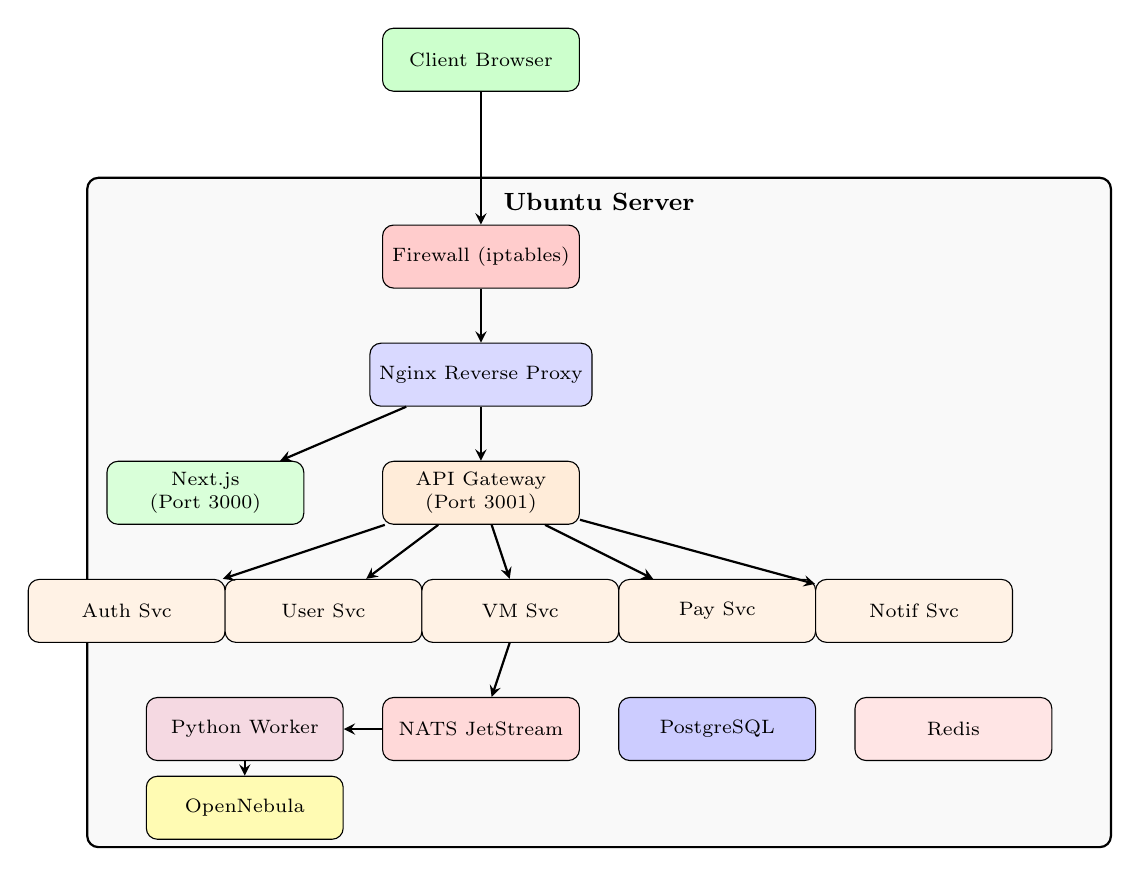
\begin{tikzpicture}[
  box/.style={draw, rounded corners, minimum width=2.5cm, minimum height=0.8cm, align=center, font=\scriptsize},
  container/.style={draw, dashed, rounded corners, inner sep=0.3cm},
  arrow/.style={->, thick, >=stealth}
]
  % Client
  \node[box, fill=green!20] (client) at (0, 4) {Client Browser};
  
  % Server boundary
  \draw[thick, rounded corners, fill=gray!5] (-5, -6) rectangle (8, 2.5);
  \node[font=\small\bfseries] at (1.5, 2.2) {Ubuntu Server};
  
  % Firewall
  \node[box, fill=red!20] (fw) at (0, 1.5) {Firewall (iptables)};
  
  % Docker containers
  \node[box, fill=blue!15] (nginx) at (0, 0) {Nginx Reverse Proxy};
  
  \node[box, fill=green!15] (next) at (-3.5, -1.5) {Next.js\\(Port 3000)};
  \node[box, fill=orange!15] (gate) at (0, -1.5) {API Gateway\\(Port 3001)};
  
  \node[box, fill=orange!10] (auth) at (-4.5, -3) {Auth Svc};
  \node[box, fill=orange!10] (usersvc) at (-2, -3) {User Svc};
  \node[box, fill=orange!10] (vmsvc) at (0.5, -3) {VM Svc};
  \node[box, fill=orange!10] (paysvc) at (3, -3) {Pay Svc};
  \node[box, fill=orange!10] (notifsvc) at (5.5, -3) {Notif Svc};
  
  \node[box, fill=purple!15] (worker) at (-3, -4.5) {Python Worker};
  \node[box, fill=red!15] (nats) at (0, -4.5) {NATS JetStream};
  \node[box, fill=blue!20] (pg) at (3, -4.5) {PostgreSQL};
  \node[box, fill=red!10] (redis) at (6, -4.5) {Redis};
  
  % OpenNebula
  \node[box, fill=yellow!30] (one) at (-3, -5.5) {OpenNebula};
  
  % Arrows
  \draw[arrow] (client) -- (fw);
  \draw[arrow] (fw) -- (nginx);
  \draw[arrow] (nginx) -- (next);
  \draw[arrow] (nginx) -- (gate);
  \draw[arrow] (gate) -- (auth);
  \draw[arrow] (gate) -- (usersvc);
  \draw[arrow] (gate) -- (vmsvc);
  \draw[arrow] (gate) -- (paysvc);
  \draw[arrow] (gate) -- (notifsvc);
  \draw[arrow] (vmsvc) -- (nats);
  \draw[arrow] (nats) -- (worker);
  \draw[arrow] (worker) -- (one);
\end{tikzpicture}
\caption{Deployment architecture}
\label{fig:deployment}
\end{figure}

\subsection{Network Topology}

\begin{figure}[H]
\centering
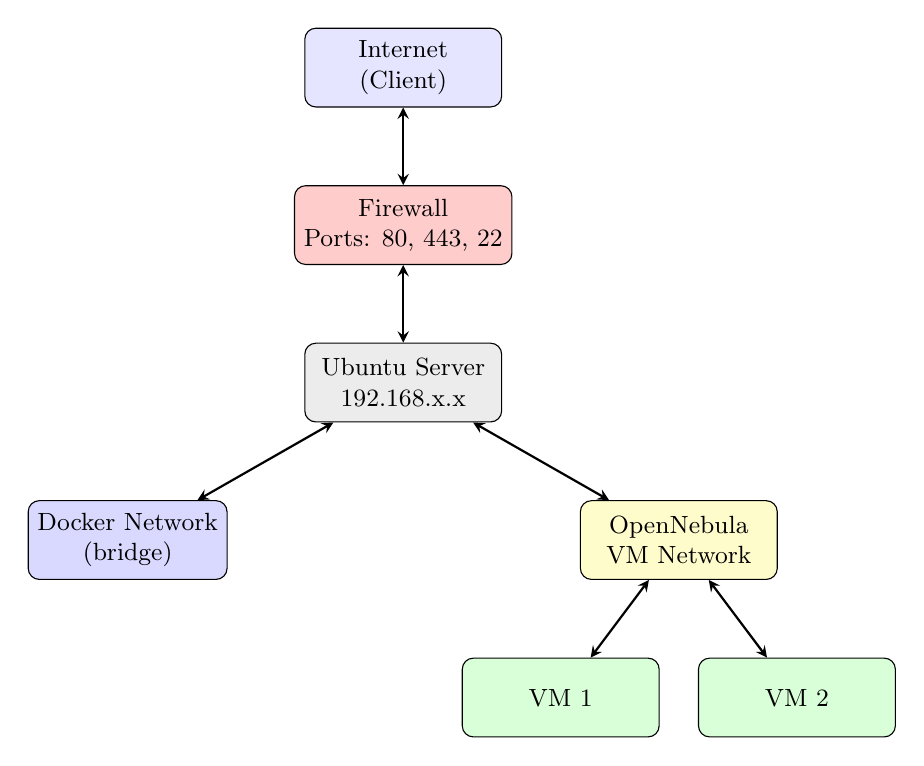
\begin{tikzpicture}[
  box/.style={draw, rounded corners, minimum width=2.5cm, minimum height=1cm, align=center, font=\small},
  arrow/.style={<->, thick, >=stealth}
]
  % Internet
  \node[box, fill=blue!10] (internet) at (0, 3) {Internet\\(Client)};
  
  % Firewall
  \node[box, fill=red!20] (fw) at (0, 1) {Firewall\\Ports: 80, 443, 22};
  
  % Server
  \node[box, fill=gray!15] (server) at (0, -1) {Ubuntu Server\\192.168.x.x};
  
  % Docker Network
  \node[box, fill=blue!15] (docker) at (-3.5, -3) {Docker Network\\(bridge)};
  
  % VM Network
  \node[box, fill=yellow!20] (vmnet) at (3.5, -3) {OpenNebula\\VM Network};
  
  % VMs
  \node[box, fill=green!15] (vm1) at (2, -5) {VM 1};
  \node[box, fill=green!15] (vm2) at (5, -5) {VM 2};
  
  \draw[arrow] (internet) -- (fw);
  \draw[arrow] (fw) -- (server);
  \draw[arrow] (server) -- (docker);
  \draw[arrow] (server) -- (vmnet);
  \draw[arrow] (vmnet) -- (vm1);
  \draw[arrow] (vmnet) -- (vm2);
\end{tikzpicture}
\caption{Network topology diagram}
\label{fig:network-topology}
\end{figure}

\subsection{Implementation Screenshots}

\begin{figure}[H]
\centering
\fbox{\parbox{0.9\textwidth}{\centering\vspace{3cm}\textit{Insert deployed platform screenshot (complete dashboard)}\vspace{3cm}}}
\caption{Deployed platform — User dashboard}
\label{fig:deployed-dashboard}
\end{figure}

\begin{figure}[H]
\centering
\fbox{\parbox{0.9\textwidth}{\centering\vspace{3cm}\textit{Insert Docker containers running screenshot}\vspace{3cm}}}
\caption{Docker containers running on the server}
\label{fig:docker-running}
\end{figure}

\subsection{Sprint 8 Review}

At the end of Sprint 8:
\begin{itemize}
  \item All services deployed via Docker Compose on Ubuntu Server.
  \item Production-optimized Docker builds (multi-stage).
  \item Nginx reverse proxy configured.
  \item Final smoke tests passed on deployed platform.
  \item Report completed and reviewed.
  \item Presentation slides and demo script prepared.
\end{itemize}

% ============================================================
\section{Conclusion}

In this final chapter, we completed the platform development with notification features, thorough testing, and full deployment. Sprint 7 ensured the platform's quality through integration testing and UI refinements. Sprint 8 delivered the production deployment with Docker, configured the server with proper security, and prepared all project deliverables.

The CloudVM platform is now fully functional, allowing users to create and manage virtual machines through a modern web interface, with secure authentication, quota management, and payment processing.

% ============================================================
% GENERAL CONCLUSION (to be added to main.tex)
% ============================================================
% Uncomment the following in main.tex at the end:

% \chapter*{General Conclusion}
% \addcontentsline{toc}{chapter}{General Conclusion}
% 
% Throughout this project, we designed and developed CloudVM — a comprehensive 
% cloud virtual machine management platform. The project was carried out within 
% the Readdly startup over a period of 8 weeks, following the Agile/Scrum methodology.
%
% The platform successfully delivers the following capabilities:
% \begin{itemize}
%   \item A modern, responsive web interface for VM management
%   \item Secure authentication with JWT and role-based access control
%   \item Full VM lifecycle management (create, start, stop, reboot, delete)
%   \item Web-based CLI terminal access to VMs (Phase~1) using xterm.js and WebSocket SSH proxy
%   \item SSH key management for secure VM authentication
%   \item Asynchronous processing through a Python worker and NATS JetStream
%   \item Quota enforcement and payment processing for plan upgrades
%   \item Server-side security with OpenNebula and firewall configuration
% \end{itemize}
%
% This project allowed us to apply the knowledge gained during our studies at 
% ISET Mahdia in a real-world context. We gained hands-on experience with 
% microservices architecture, containerization, cloud computing, and modern 
% web development practices.
%
% As future improvements, we envision:
% \begin{itemize}
%   \item \textbf{Phase~2 --- Full Desktop Streaming:} Upgrading VM access from the current CLI terminal to full graphical desktop streaming using VNC/noVNC, allowing users to interact with the VM's GUI (Windows desktop, Linux desktop environment) directly in the browser
%   \item Implementing auto-scaling and load balancing
%   \item Adding support for Kubernetes-based container orchestration
%   \item Deploying on public cloud infrastructure for wider accessibility
%   \item Adding more payment providers and subscription models
% \end{itemize}
